\documentclass[tikz]{standalone}

\colorlet{FilledSurface}{blue!20}
\colorlet{FilledSurfaceGroupOne}{blue!20}
\colorlet{FilledSurfaceGroupTwo}{red!20}
\colorlet{FilledSurfaceGroupThree}{green!20}
\colorlet{FilledSurfaceGroupFour}{magenta!20}
\colorlet{FormulaBackground}{green!10}
\colorlet{FormulaFrame}{green}


\usetikzlibrary{calc, angles}

\begin{document}
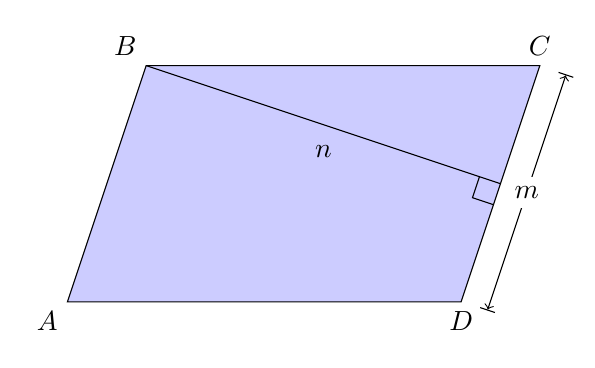
\begin{tikzpicture}

\coordinate (A) at (0, 0);
\coordinate (B) at (1, 3);
\coordinate (C) at (6, 3);
\coordinate (D) at (5, 0);
\draw[fill = FilledSurfaceGroupOne]
    (A) node[below left]{$A$}
    -- (B) node[above left]{$B$}
    -- (C) node[above]{$C$}
    -- (D) node[below]{$D$}
    -- cycle;

\coordinate (E) at ($(C)!(B)!(D)$);
\draw (B) -- node[below=4pt] {$n$} (E);
\path pic [draw, angle radius = 8pt] {right angle = B--E--D};

\draw[color = black,|<->|] ($(D)!10pt!-90:(C)$) to node [fill=white, midway] {$m$} ($(C)!10pt!90:(D)$);

\end{tikzpicture}
\end{document}


